\documentclass[compress]{beamer}
\usetheme{Warsaw}
\usecolortheme{crane}
\usepackage[utf8]{inputenc}
\usepackage[portuguese]{babel}
\usepackage{url}
\usepackage{tikz}
\usetikzlibrary{arrows}
\usetikzlibrary{arrows}
\usepackage{default}
\usepackage{amsmath}
\usepackage{amsfonts}
\usepackage{amssymb}

% Algumas definições %%%
\def\term#1{{\sc #1}}   % IR terms in examples not index terms!
\def\query#1{{\sf #1}}
\def\oper#1{{\sc #1}} % AND, OR, NOT
%%%%%%%%%%%%%%%%%%%%%%%%

\title[Coelho: Introdução]
{Introdução à Recuperação de Informações\\
\large \url{https://github.com/fccoelho/curso-IRI}\\[0.5cm]
IRI 1: Introdução}

\author [Coelho F.C. \& Souza R.R.]{ Flávio Codeço Coelho}

\institute [EMAp, FGV]{Escola de Matemática Aplicada,   Fundação Getúlio Vargas}
\date


\begin{document}

\begin{frame}
\titlepage
\end{frame}

\begin{frame}[fragile]
\frametitle{Sumário da Aula}
\tableofcontents
\end{frame}

\section{Introdução}
\begin{frame}[fragile]
\frametitle{Definição}
\begin{quote}
 Recuperação de informação pode ser definida como a técnica e a arte de \alert<2,7>{encontrar} conteúdo em \alert<3,7>{grandes coleções} \alert<4,7>{não (ou pouco) estruturadas}
 de \alert<5,7>{documentos} (em formatos digitais) de forma a satisfazer nossas \alert<6,7>{necessidades informacionais}\footnote{adaptado de Hinrich Schütze}.
\end{quote} 
\end{frame}

\section{Estrutura do Curso}

\begin{frame}[fragile]
\frametitle{Mecânica do Curso}
\begin{itemize}[<+->]
 \item Foco na Recuperação de informação em coleções de texto.
 \item Exercícios exigirão conhecimentos de programação em Python
 \item Avaliação baseada em mini-projetos (um projeto a cada duas semanas)
 \item Projetos serão desenvolvidos em duplas rotatórias, ou seja, cada par de alunos só poderá trabalhar em um projeto.
 \item Dados e infraestrutura computacional serão fornecidos pela escola sempre que necessário
 
\end{itemize}
\end{frame}

\begin{frame}[fragile]
\frametitle{Contéudo}
Este curso se restringirá à exploração e aplicação de modelos matemáticos de recuperação de informação
\begin{itemize}[<+->]
 \item Modelos Booleanos
  \begin{itemize}
    \item Fuzzy
    \item Modelo Booleano extendido
  \end{itemize}
 \item Modelos Vetoriais
  \begin{itemize}
    \item Espaços vetoriais
    \item Indexação semântica latente
    \item Classificação
    \item Clusterização
  \end{itemize}
 \item Modelos Probabilísticos
  \begin{itemize}
    \item Redes Bayesianas
    \item Graphical Models
    \item Belief Networks
  \end{itemize}
\end{itemize}
\end{frame}

\section{Avaliando a Recuperação}
\begin{frame}[fragile]
\frametitle{Quão boa é nossa recuperação?}
Antes de desenvolver qualquer estratégia de recuperação precisamos definir nossa meta e uma métrica de qualidade.
\begin{itemize}[<+->]
 \item A meta depende da necessidade informacional
 \item Existem algumas métricas classicas de qualidade
\end{itemize}
\end{frame}

\subsection{Revocação e Precisão}

\begin{frame}[fragile]
\frametitle{Precisão e Revocação(Recall)}
Seja $R$ um conjunto de documentos relevantes e $|R|$ o número de documentos neste conjunto. Uma requisiçã de informação $I$, gera um conjunto $A$ contendo $|A|$ documentos em resposta. Seja $|R_a|$ o número de documentos da interseção entre $R$ e $A$

Podemos definir revocação como:

\begin{columns}
 \column{3cm}
  \begin{equation*}
  Rev = \frac{|R_a|}{|R|}
  \end{equation*}
  \column{3cm}
  \begin{figure}[h!]
    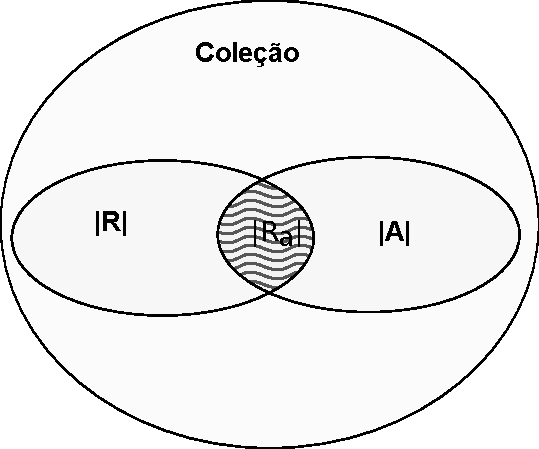
\includegraphics[width=3cm]{./recall.pdf}
    % recall.pdf: 259x216 pixel, 72dpi, 9.14x7.62 cm, bb=0 0 259 216
  \end{figure}
\column{4cm}
  \begin{equation*}
    Precis\tilde{a}o = \frac{|R_a|}{|A|}
  \end{equation*} 
\end{columns}
\end{frame}

\begin{frame}%[fragile]
\frametitle{Na Prática}
Seja $R_q = \{d_3,d_5,d_9,d_{25},d_{39},d_{44},d_{56},d_{71},d_{89},d_{123}\}$ o conjunto de documentos relevantes para uma consulta $q$.

Ordenando o conjunto $A_q$ de respostas a $q$ em ordem decrescente de relevância, temos:

\begin{block}{Resultados ordenados}
\begin{tabular*}{}{llll}
\hline
Ordem & Resultado & Precisão & Revocação\\\hline
1 & $\mathbf{d_{123}}$ & 100\% & 10\%\\
2 & $d_{84}$ & 50\% & 10\%\\\hline
3 & $\mathbf{d_{56}}$ & 66\% & 20\%\\
4 & $d_6$ & 50\% & 20\%\\
5 & $d_8$ & 40\% & 20\%\\
6 & $\mathbf{d_9}$ & 50\% & 30\%\\
\end{tabular*}
\end{block}
\end{frame}

\begin{frame}[fragile]
\frametitle{Problemas}
\begin{itemize}
 \item Conjunto $|R|$ em situações reais pode ser difícil ou impossível de determinar.
  \item Revocação e Precisão são medidas correlacionadas.
\item visão muito simplista sobre a qualidade da recuperação.
\end{itemize}
\end{frame}

\subsection{Outras métricas}

\begin{frame}[fragile]
\frametitle{Média Harmônica}
Como precisão e revocação são medidas correlacionadas, podemos buscar integrá-las em uma mesma medida.
\begin{block}{Média Harmônica}
\begin{equation*}
 F(j)=\frac{2}{\frac{1}{r_j}+\frac{1}{P_j}}
\end{equation*}
\end{block}
onde $r_j$ e $P_j$ são a revocação e a precisão do j-ésimo documento rankeado.

$F(j)$ assume valores no intervalo $\left[ 0,1\right]$, sendo $0$ quando nenhum documento relevante for recuperado e 1 quando todos os documentos recuperados forem relevantes.
\end{frame}

\begin{frame}[fragile]
\frametitle{Medida E}
\begin{block}{$E(j)$}
$$
 E(j)=1-\frac{1+b^2}{\frac{b^2}{r_j}+\frac{1}{P_j}}
$$
\end{block}

Onde $b$ é um parâmetro the indica a importância relativa da revocação e da precisão. Quando $b=1$, $E$ é o complemento da média harmônica. Quando $b<1$, damos mais peso à precisão e quando $b>1$ damos mais peso à revocação.

\end{frame}

\begin{frame}[fragile]
\frametitle{Medidas Subjetivas}
Seja $U$ um subconjunto de $R$ que é do conhecimento do usuário. $|U|$ é o número de documentos neste conjunto. Seja $|R_k|$ o número de documentos da interseção entre $A$ e $U$, e $|R_u|$ o número de documentos pertencentes a $A$ mas não a $U$, i.e., $A-U$
\begin{block}{Cobertura e Novidade}
$$
Cobertura = \frac{|R_k|}{|U|}
$$
$$
Novidade = \frac{|R_u|}{|R_u|+|R_k|}
$$
\end{block}
\end{frame}

\section{Recuperação Booleana}

\begin{frame}[fragile]
\frametitle{Recuperação Booleana}
Modelo de recuperação no qual podemos construir consultas na forma de uma expressão booleana, ou seja, os termos de busca são combinados com operadores \oper{and}, \oper{or} e \oper{or}. este modelo vê cada documento como um simples conjunto de palavras.
\end{frame}

\begin{frame}
\frametitle{Dados não estruturados de 1650}
\begin{itemize}[<+->]
\item Que peças de Shakepeare contêm as palavras
\term{Brutus}
\oper{and} 
\term{Caesar}, mas 
\oper{not} 
\term{Calpurnia}?
\item Poderíamos fazer um  grep em todas as peças de Shakespeare's por 
\term{Brutus}
e \term{Caesar}, e então remover as linhas contendo  
\term{Calpurnia}.
\item \green{Porque o grep não é a solução?}
\visible<4->{
\begin{itemize}
\item Lento (para grandes coleções)
\item grep é orientado a linhas, RI é orientada a documentos
\item ``\oper{not} \term{Calpurnia}'' não é trivial 
\item Outras operações, tais como por exemplo: encontrar a palavra \term{Romans}
  proxima da palavra \term{countryman}) não é factivel.
\item Recuperação Rankeada (melhores documentos) 
\end{itemize}}
\end{itemize}
\end{frame}

\begin{frame}[shrink=15]
\frametitle{Matriz de incidência Termo-Documento}

\begin{tabular}{@{}lccccccc@{}}
 & Anthony  & Julius & The  & Hamlet &
 Othello & Macbeth & \ldots \\
 & and  & Caesar & Tempest &  &  &  &  \\
 & Cleopatra \\
\term{Anthony} &    1 & 1 & 0 & 0 & 0 & 1 & \\
\term{Brutus} &     1 & 1 & 0 & 1 & 0 & 0 & \\
\term{Caesar} &     1 & 1 & 0 & 1 & 1 & 1 & \\
\term{Calpurnia} &  0 & \alert<2>{1} & \alert<3>{0} & 0 & 0 & 0 & \\
\term{Cleopatra} &  1 & 0 & 0 & 0 & 0 & 0 & \\
\term{mercy} &      1 & 0 & 1 & 1 & 1 & 1 & \\
\term{worser} &     1 & 0 & 1 & 1 & 1 & 0 & \\
\ldots
\end{tabular}

\alert<2>{
Elemento é is 1 se o termo ocorre. Exemplo: \term{Calpurnia} ocorre
em \emph{Julius Caesar}.}

\alert<3>{
Elemento é 0 se o termo não ocorre. Exemplo: \term{Calpurnia}
não ocorre em \emph{The tempest}.
}
\end{frame}

\begin{frame}
\frametitle{Vetores de Incidencia }
\begin{itemize}
\item Então temos um 0/1 vector para cada termo.
\item Para responder à consulta
\term{Brutus}
\oper{and} 
\term{Caesar}
\oper{and} 
\oper{not} 
\term{Calpurnia}:
\visible<2>{\begin{itemize}
\item Basta tomarmos os vetores para  
\term{Brutus},
\term{Caesar}, e
\term{Calpurnia}
\item tomar o complemento do vetor para \term{Calpurnia}
\item fazer um (bitwise) \oper{and} dos os três vetores
\item 110100 \oper{and} 110111 \oper{and} 101111 = 100100
\end{itemize}}
\end{itemize}
\end{frame}

\subsection{Indices invertidos}

\begin{frame}
\frametitle{Coleções maiores}
\begin{itemize}[<+->]
\item Considere $N= 10^6$ documentos, cada um com cerca de 1000 tokens
\item $\Rightarrow$ totalizando $10^9$ tokens
\item Assumindo uma média de 6 bytes por token, incluindo espaços e pontuação
$\Rightarrow$ tamanho do \emph{corpus} $6 \cdot
  10^9=$ 6~GB
\item Assumindo que existam $M=500{,}000$ termos distintos na coleção
\item (Note a diferença entre termo e token )
\end{itemize}
\end{frame}

\begin{frame}
\frametitle{Impossível construir a matriz de incidência}
\begin{itemize}[<+->]
\item 
 $M=500{,}000 \times
10^6 = $ meio trilhão de 0s e 1s.
\item Mas esta matriz não tem mais que 1 bilhão de 1s. 
\begin{itemize}[<+->]
\item Extremamente esparsa.
\end{itemize}
\item Qual seria uma representação melhor?
\begin{itemize}[<+->]
\item Registrar apenas os 1s.
\end{itemize}
\end{itemize}
\end{frame}

\begin{frame}
\frametitle{Índice Invertido}

Para cada termo $t$, armazenamos uma lista com os documentos em que este ocorre.

\bigskip

\begin{tabular}{|c|c|r|r|r|r|r|r|r|r|r|}
\cline{1-1}\cline{3-10}
\term{Brutus} & $\longrightarrow$ & 1 & 2 & 4 & 11 & 31 & 45 & 173 & 174 \\ \cline{1-1}\cline{3-10}
\multicolumn{8}{l}{} \\ \cline{1-1}\cline{3-11}
\term{Caesar} & $\longrightarrow$ & 1 & 2 & 4 & 5 & 6 & 16 & 57 & 132 & \ldots \\ \cline{1-1}\cline{3-11}
\multicolumn{8}{l}{} \\ \cline{1-1}\cline{3-6}
\term{Calpurnia} & $\longrightarrow$ & 2 & 31 & 54 & 101 \\
\cline{1-1}\cline{3-6} \multicolumn{8}{l}{}  \\
% The multicolumn{1}'s below suppress the vertical lines....
\multicolumn{1}{c}{$\vdots$} \\
\multicolumn{1}{c}{$\underbrace{\phantom{\mbox{Calpurnia}}}$} &
\multicolumn{1}{c}{} &
\multicolumn{9}{c}{$\underbrace{\phantom{\mbox{Calpurnia Calpurnia
Calpurnia Caesar hath}}}$} \\
\multicolumn{1}{c}{\alert<2>{\textbf{dicionário}}} &
\multicolumn{1}{c}{} & \multicolumn{9}{c}{\alert<3>{\textbf{postings}}}
\end{tabular}

\end{frame}



\begin{frame}
\frametitle{Construindo um Índice Invertido}
\begin{enumerate}
\item Junte os documentos a serem indexados:\\[0.2ex]
\framebox{\weestrut Friends, Romans, countrymen.}
\framebox{\weestrut So let it be with Caesar} \ldots
\item Tokenize o texto, transformando cada documento em uma lista de tokens:\\[0.2ex]
\framebox{\weestrut Friends} \framebox{\weestrut Romans}
\framebox{\weestrut countrymen} \framebox{\weestrut So} \ldots
\item Realize um pré-processamento linguístico, produzindo uma lista de termos normalizados, que serão os termos indexados:
\framebox{\weestrut friend} \framebox{\weestrut roman}
  \framebox{\weestrut countryman} \framebox{\weestrut so} \ldots
\item Indexe os documentos em que cada termo ocorre criando um índice invertido, consistindo de um dicionário e postings.
\end{enumerate}
\end{frame}



\end{document}
